\documentclass[10pt,a4paper,twoside]{article}
\usepackage[utf8]{inputenc}
\usepackage[english]{babel}
\usepackage{graphicx}
\usepackage{geometry}
\geometry{
 a4paper,
 total={170mm,257mm},
 left=20mm,
 top=20mm,
 }
\usepackage[dvipsnames]{xcolor}
\usepackage{tikz}
\usetikzlibrary{arrows,automata,shapes}
\tikzstyle{decision} = [diamond, draw, fill=blue!20, text width=4.5em, text badly centered, node distance=2.5cm, inner sep=0pt]
\tikzstyle{block} = [rectangle, draw, fill=blue!20, text width=5em, text centered, rounded corners, minimum height=4em]
\tikzstyle{line} = [draw, very thick, color=black!50, -latex']
\tikzstyle{cloud} = [draw, ellipse,fill=red!20, node distance=2.5cm,minimum height=2em]

\author{David Lanzendörfer}
\begin{document}
\begin{abstract}    
	This process is licensed under the Libre Silicon public license; you can redistribute it and/or modify it under the terms of the Libre Silicon public license
	as published by the Libre Silicon alliance, either version 2 of the License, or (at your option) any later version.

	This design is distributed in the hope that it will be useful, but WITHOUT ANY WARRANTY; without even the implied warranty of MERCHANTABILITY or FITNESS FOR A PARTICULAR PURPOSE.
	See the Libre Silicon Public License for more details. \\

	This is the specification of the free silicon manufacturing standard for manufacturing the ls018\footnotemark standard logic cells and related free technology nodes from the LibreSilicon project.
	\footnotetext[1]{https://github.com/leviathanch/ls018}
\end{abstract}

\section{Well}
\begin{tabular}{c c}
	\hline 
	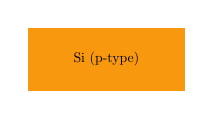
\begin{tikzpicture}[node distance = 3cm, auto, thick,scale=0.5, every node/.style={transform shape}]
		% substrate
		\fill[YellowOrange] (0,0) rectangle (4,1.6);
		\node at (2,0.8) {Si (p-type)};
	\end{tikzpicture} &
	We start with a p-type silicon wafer
	\\ \hline 
	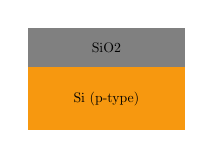
\begin{tikzpicture}[node distance = 3cm, auto, thick,scale=0.5, every node/.style={transform shape}]
		% substrate
		\fill[YellowOrange] (0,0) rectangle (4,1.6);
		\node at (2,0.8) {Si (p-type)};
		% oxide
		\fill[gray] (0,1.6) rectangle (4,2.6);
		\node at (2,2.1) {SiO2};
	\end{tikzpicture} &
	We grow an oxide layer of approximately 1000 angstrom thickness (see documentation)
	\\ \hline 
	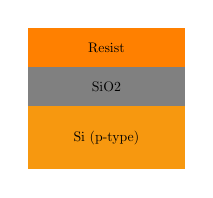
\begin{tikzpicture}[node distance = 3cm, auto, thick,scale=0.5, every node/.style={transform shape}]
		% substrate
		\fill[YellowOrange] (0,0) rectangle (4,1.6);
		\node at (2,0.8) {Si (p-type)};
		% oxide
		\fill[gray] (0,1.6) rectangle (4,2.6);
		\node at (2,2.1) {SiO2};
		% resist
		\fill[orange] (0,2.6) rectangle (4,3.6);
		\node at (2,3.1) {Resist};
	\end{tikzpicture} &
	We thin film deposit a layer of resist
	\\ \hline
	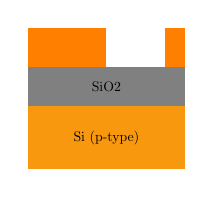
\begin{tikzpicture}[node distance = 3cm, auto, thick,scale=0.5, every node/.style={transform shape}]
		% substrate
		\fill[YellowOrange] (0,0) rectangle (4,1.6);
		\node at (2,0.8) {Si (p-type)};
		% oxide
		\fill[gray] (0,1.6) rectangle (4,2.6);
		\node at (2,2.1) {SiO2};
		% resist 1
		\fill[orange] (0,2.6) rectangle (2,3.6);
		% resist 2
		\fill[orange] (3.5,2.6) rectangle (4,3.6);
	\end{tikzpicture} &
	We expose and develop the pattern from the GDS2 layer information
	\\ \hline 
	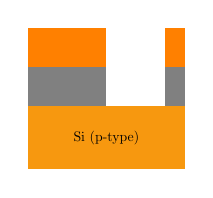
\begin{tikzpicture}[node distance = 3cm, auto, thick,scale=0.5, every node/.style={transform shape}]
		% substrate
		\fill[YellowOrange] (0,0) rectangle (4,1.6);
		\node at (2,0.8) {Si (p-type)};
		% oxide 1
		\fill[gray] (0,1.6) rectangle (2,2.6);
		% oxide 2
		\fill[gray] (3.5,1.6) rectangle (4,2.6);
		% resist 1
		\fill[orange] (0,2.6) rectangle (2,3.6);
		% resist 2
		\fill[orange] (3.5,2.6) rectangle (4,3.6);
	\end{tikzpicture} &
	We etch the 1000 angstrom oxide layer
	\\ \hline 
	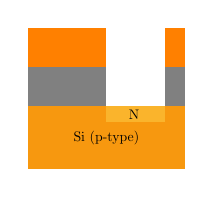
\begin{tikzpicture}[node distance = 3cm, auto, thick,scale=0.5, every node/.style={transform shape}]
		% substrate
		\fill[YellowOrange] (0,0) rectangle (4,1.6);
		\node at (2,0.8) {Si (p-type)};
		% oxide 1
		\fill[gray] (0,1.6) rectangle (2,2.6);
		% oxide 2
		\fill[gray] (3.5,1.6) rectangle (4,2.6);
		% resist 1
		\fill[orange] (0,2.6) rectangle (2,3.6);
		% resist 2
		\fill[orange] (3.5,2.6) rectangle (4,3.6);
		% well
		\fill[Dandelion] (2,1.2) rectangle (3.5,1.6);
		\node at (2.7,1.4) {N};
	\end{tikzpicture} &
	Ion implantation: Implant Phosphorus (P); n-type impurity to create N-well (see documentation)
	\\ \hline 
	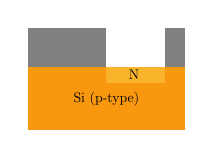
\begin{tikzpicture}[node distance = 3cm, auto, thick,scale=0.5, every node/.style={transform shape}]
		% substrate
		\fill[YellowOrange] (0,0) rectangle (4,1.6);
		\node at (2,0.8) {Si (p-type)};
		% oxide 1
		\fill[gray] (0,1.6) rectangle (2,2.6);
		% oxide 2
		\fill[gray] (3.5,1.6) rectangle (4,2.6);
		% well
		\fill[Dandelion] (2,1.2) rectangle (3.5,1.6);
		\node at (2.7,1.4) {N};
	\end{tikzpicture} &
	Remove resist
	\\ \hline 
	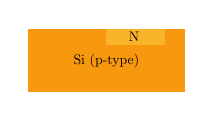
\begin{tikzpicture}[node distance = 3cm, auto, thick,scale=0.5, every node/.style={transform shape}]
		% substrate
		\fill[YellowOrange] (0,0) rectangle (4,1.6);
		\node at (2,0.8) {Si (p-type)};
		% well
		\fill[Dandelion] (2,1.2) rectangle (3.5,1.6);
		\node at (2.7,1.4) {N};
	\end{tikzpicture} &
	Remove oxide
	\\ \hline 
\end{tabular}
\end{document}